\documentclass{standalone}
\usepackage{tikz}
\usepackage{ctex,siunitx}
\setCJKmainfont{Noto Serif CJK SC}
\usepackage{tkz-euclide}
\usepackage{amsmath}
\usepackage{wasysym}
\usetikzlibrary{patterns, calc}
\usetikzlibrary {decorations.pathmorphing, decorations.pathreplacing, decorations.shapes,}
\begin{document}
\small
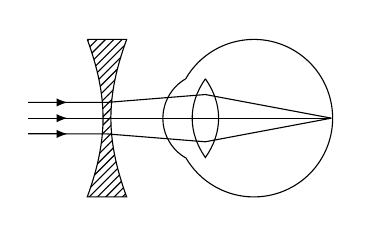
\begin{tikzpicture}[>=latex,scale=1]
  \draw (0,.5) arc (150:-150:1);
  \draw (0,.5) arc (120:240:.58);
  \draw (0.25,.5)to [bend left=35] (.25,-.5)to [bend left=35](0.25,.5) ;
  % eye end
  \draw[->] (-2,.2) to (-1.5,.2) ;
  \draw (-2,.2) --(-1,.2)--(.25,.3)--(2-.15, 0);
  \draw[->] (-2,0) to (-1.5,0) ;
  \draw (-2,0) --(.25,0)--(2-.15, 0);
  \draw[->] (-2,-.2) to (-1.5,-.2) ;
  \draw (-2,-.2) --(-1,-.2)--(.25,-.3)--(2-.15, 0);
\draw [pattern=north east lines] (-1.25, 1)--(-.75, 1)to [bend right=20]  (-.75, -1)-- (-1.25, -1)to [bend right=20]  (-1.25, 1);
\end{tikzpicture}
\end{document}